\Section{Signal Modifier Parameter Inference with cINNs}

In this chapter, the results of the network inference will be discussed in detail. Two network setups will be considered in detail: one without and one with a summary network reducing the representation of the conditions. It will be shown that the setup without a summary network results in superior predictions for which an explanation will be given. 

\Subsection{\textcolor{red}{Latent Space Distribution}}

At the end of chapter \ref{ch:deeplearning}, the loss function has been constructed in a way that the input variables should be mapped to a multivariate normal distribution with $\mu = 0$ and $\Sigma=1$. Note that thanks to the Universal Approximation Theorem, the diffeomorphic mappings in the normalizing flow represented by the GLOW coupling blocks can be approximated arbitrary well for a well-constructed network architecture and well-chosen optimization procedure. Since loss functions per se do not carry any information about the quality of the resulting mapping, the shape of the network output -- the latent space distribution -- serves as a suitable candidate to check whether there are any issues with the setup.

The latent space distribution for both networks are shown if fig. \ref{fig:latents} for the models with the lowest test loss. The distribution of the datapoints are shown in the blue histograms while a normal function with mean 0 and standard deviaiton 1 is shown in orange.

\begin{figure}[h!]
	\centering
	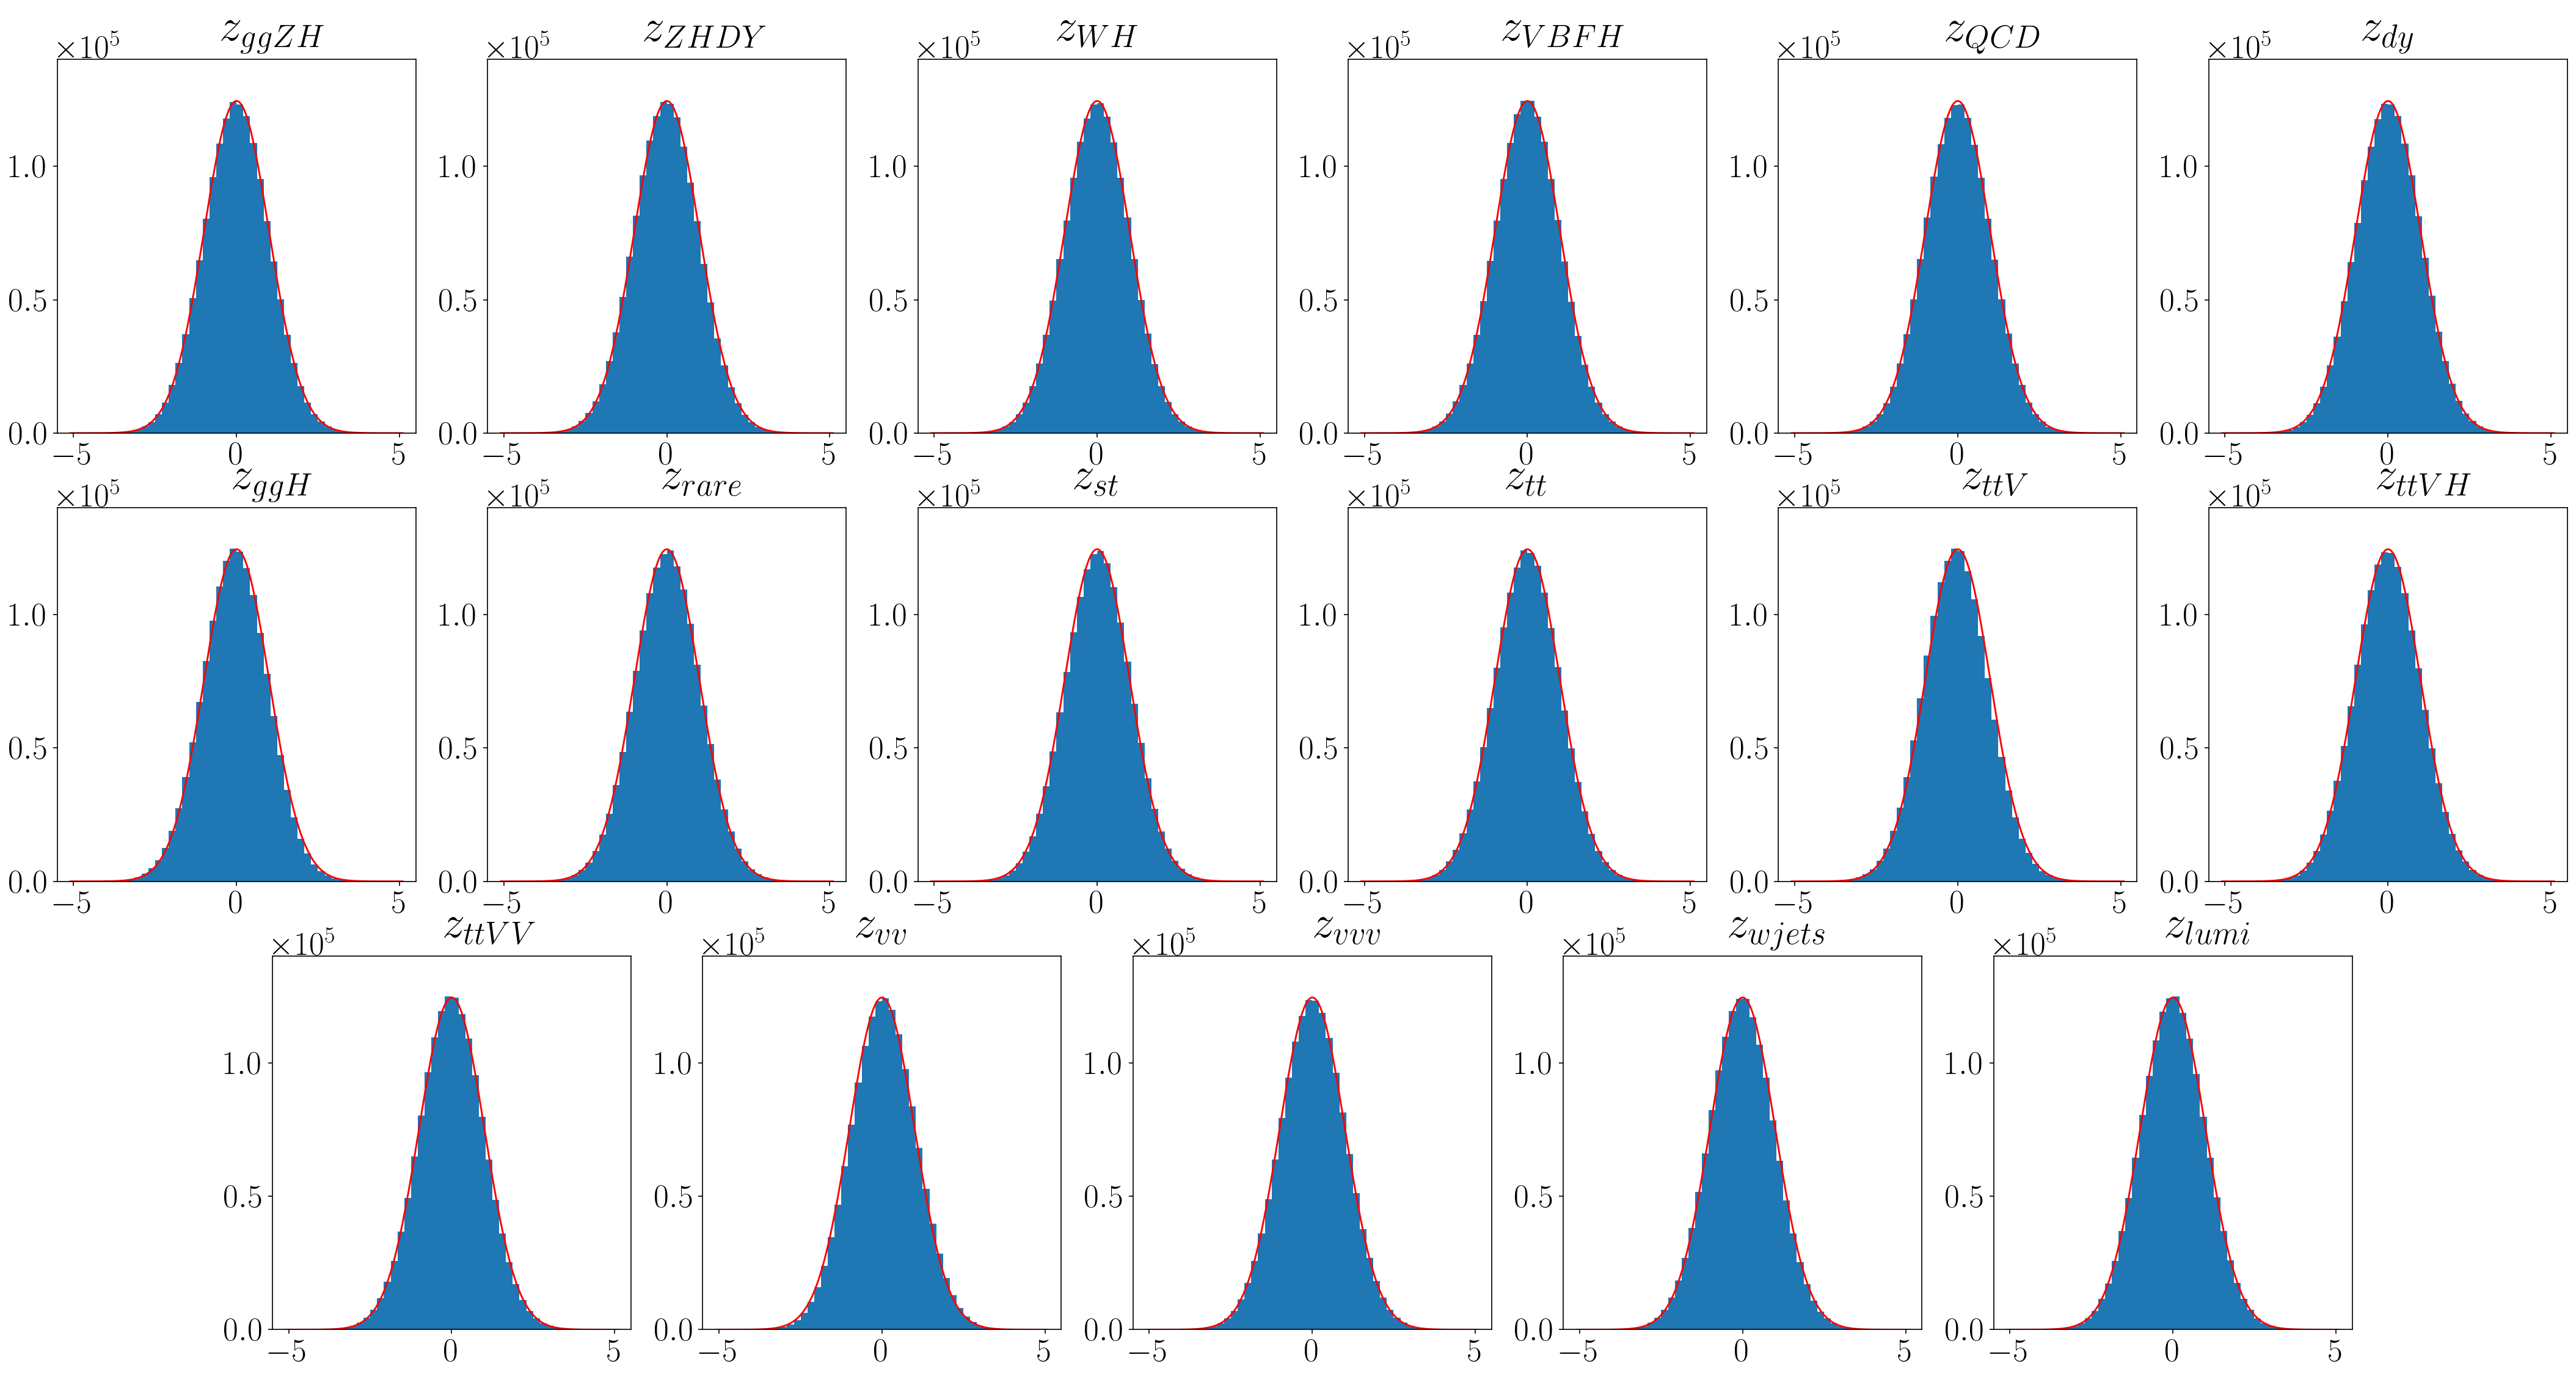
\includegraphics[width=\textwidth]{figures/inference/ls.png}
	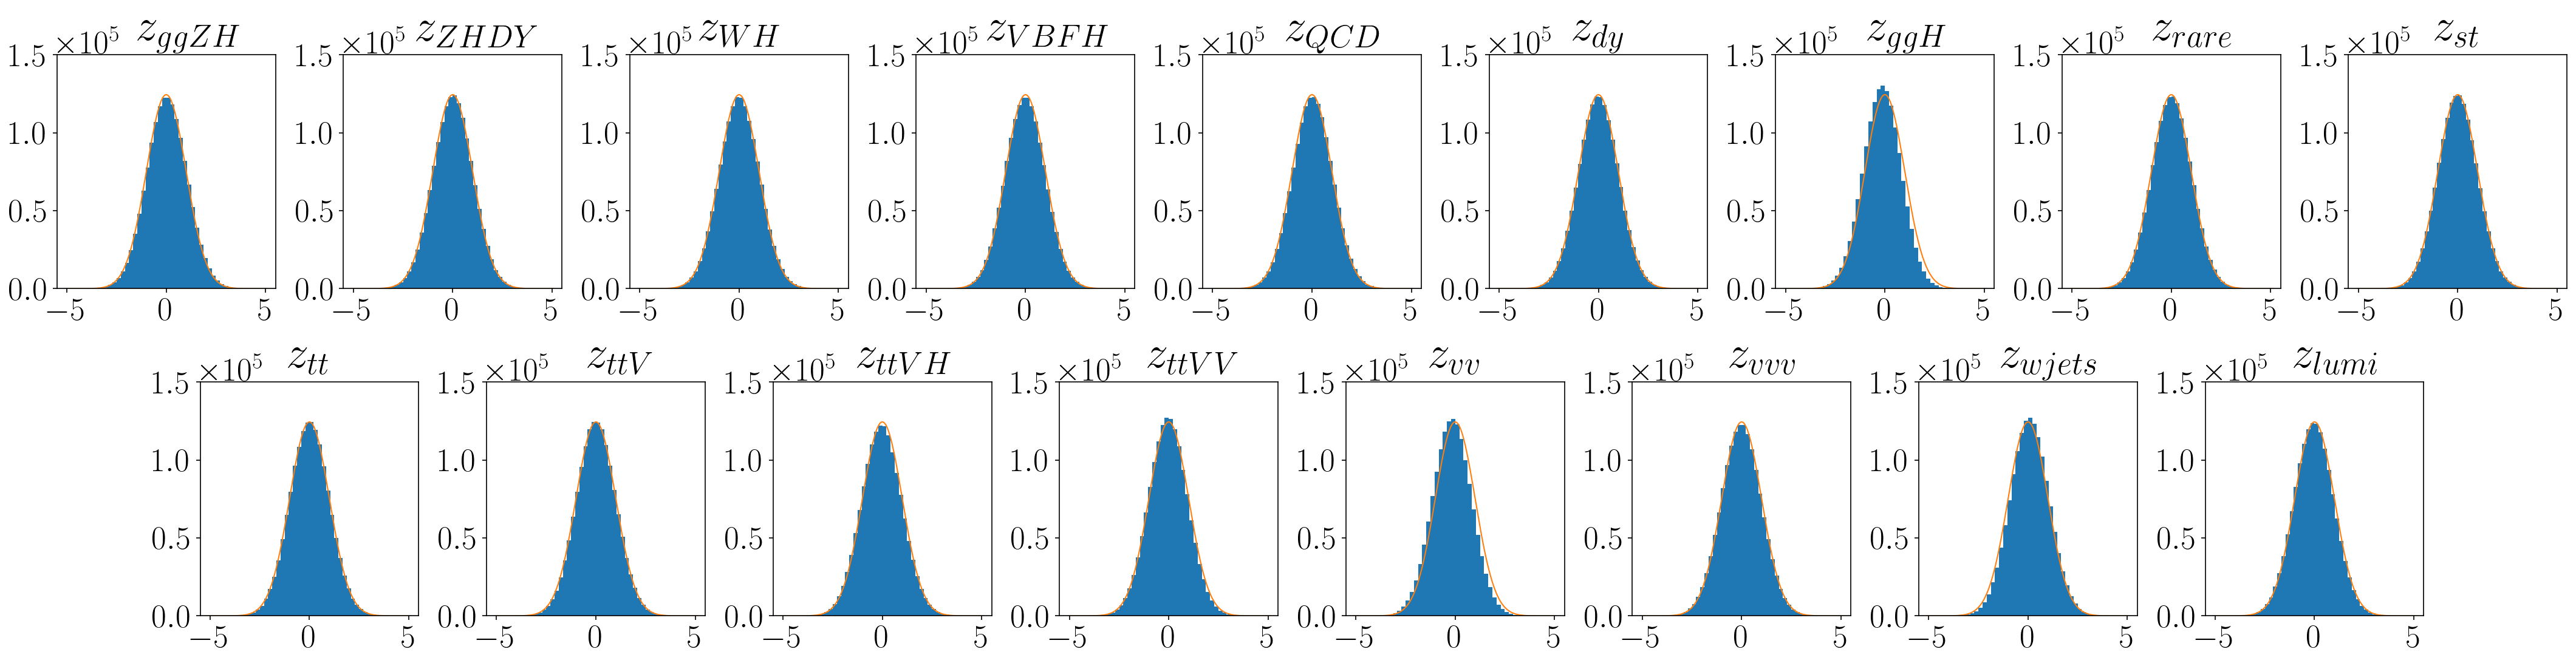
\includegraphics[width=\textwidth]{figures/inference/ls_SN.png}
	\caption{Latent space distribution for the cINN without (top) and with (bottom) a summary network.\textcolor{red}{Need to be updated!}}
	\label{fig:latents}
\end{figure}

All of the above distribution in blue are well-described by the orange curve for both networks. The network thus manages to map the input distributions to $\mathcal{N}(z; 0,1)$ well enough. The question now remains how well the cINN is capable of producing the posteriors.

\Subsection{\textcolor{red}{Calibration Curves}}

A measure of evaluating the quality of the produced posteriors are the (median) calibration errors. The calibration error for a given quantile (i.e. $q\in [0, 1]$) is defined for all histograms $N$ as

\begin{equation*}
	e_{cal}(q) = \frac{N^q_{in}}{N} - q
\end{equation*}

where $N^q_{in}$ is the number of histograms containing the true value within their $q$ quantile. For ideal posteriors, this measure is 0 for all quantiles $q$; any deviations from that signals the presence of biases and hidden correlations within the network. Naturally, no network can reproduce the ideal results, as the global optimum can only be approximated (albeit arbitrarily well). For all quantiles, the ratio of histograms are shown in fig. \ref{fig:ecals}.

\begin{figure}[h!]
	\centering
	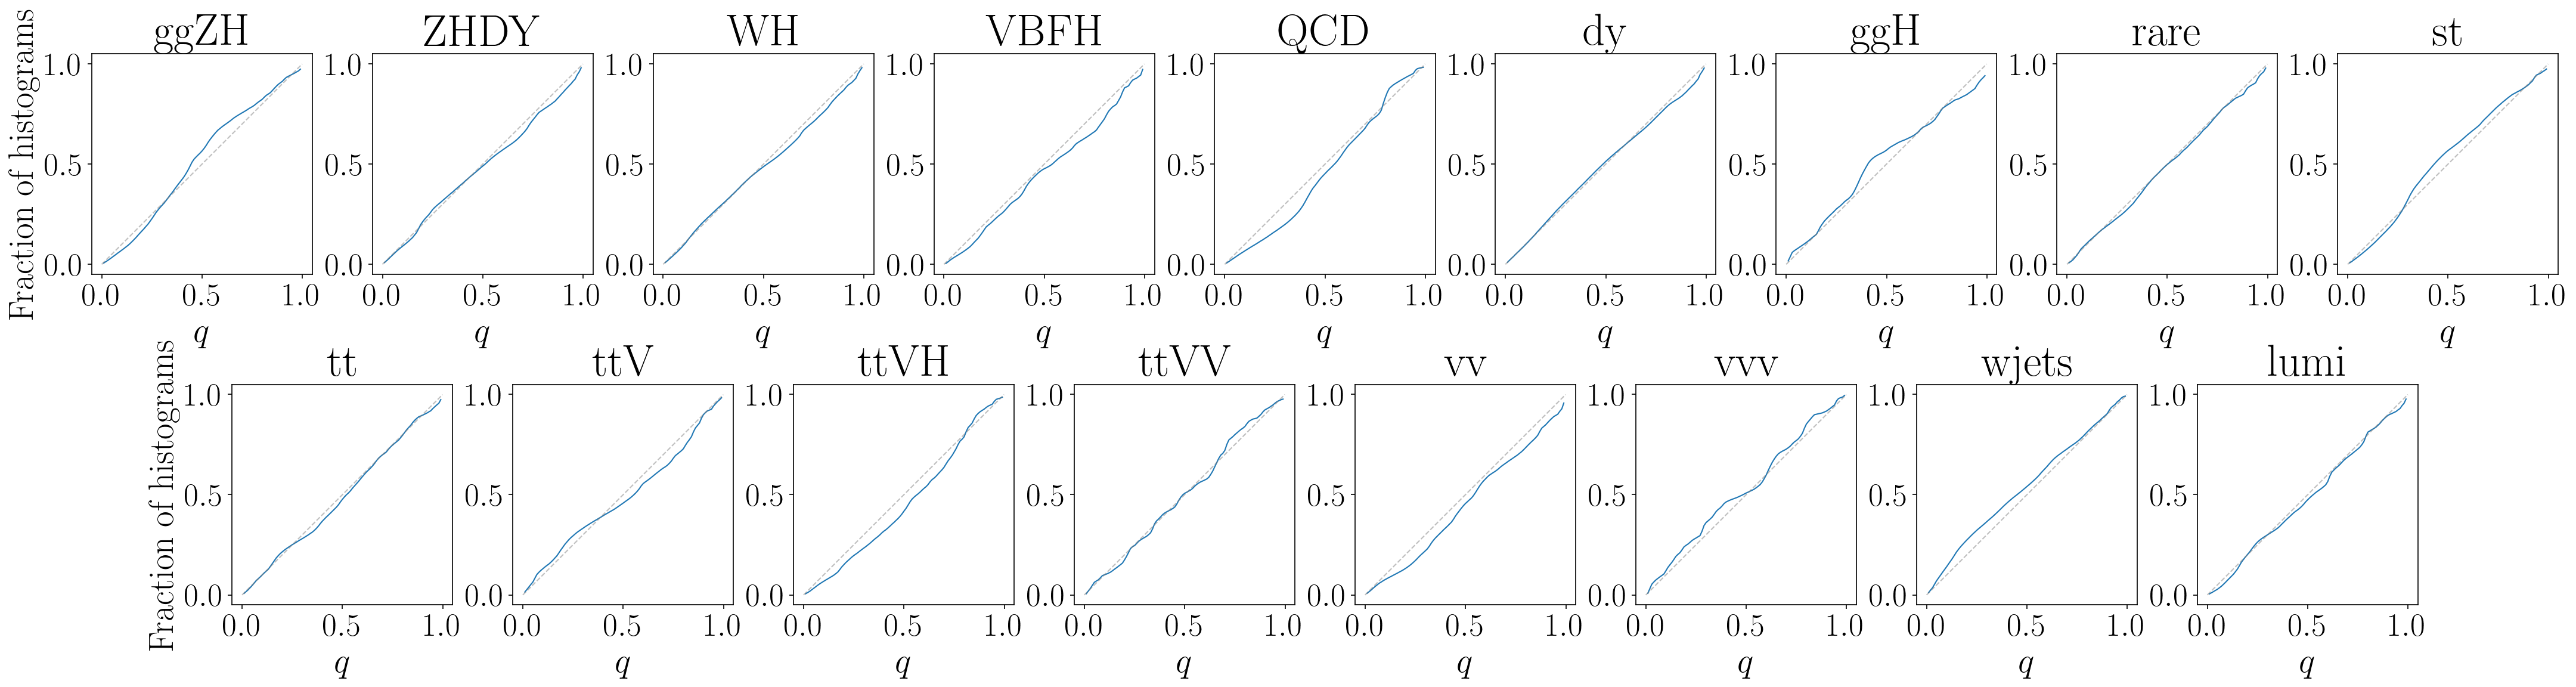
\includegraphics[width=\linewidth]{figures/inference/ecal}
	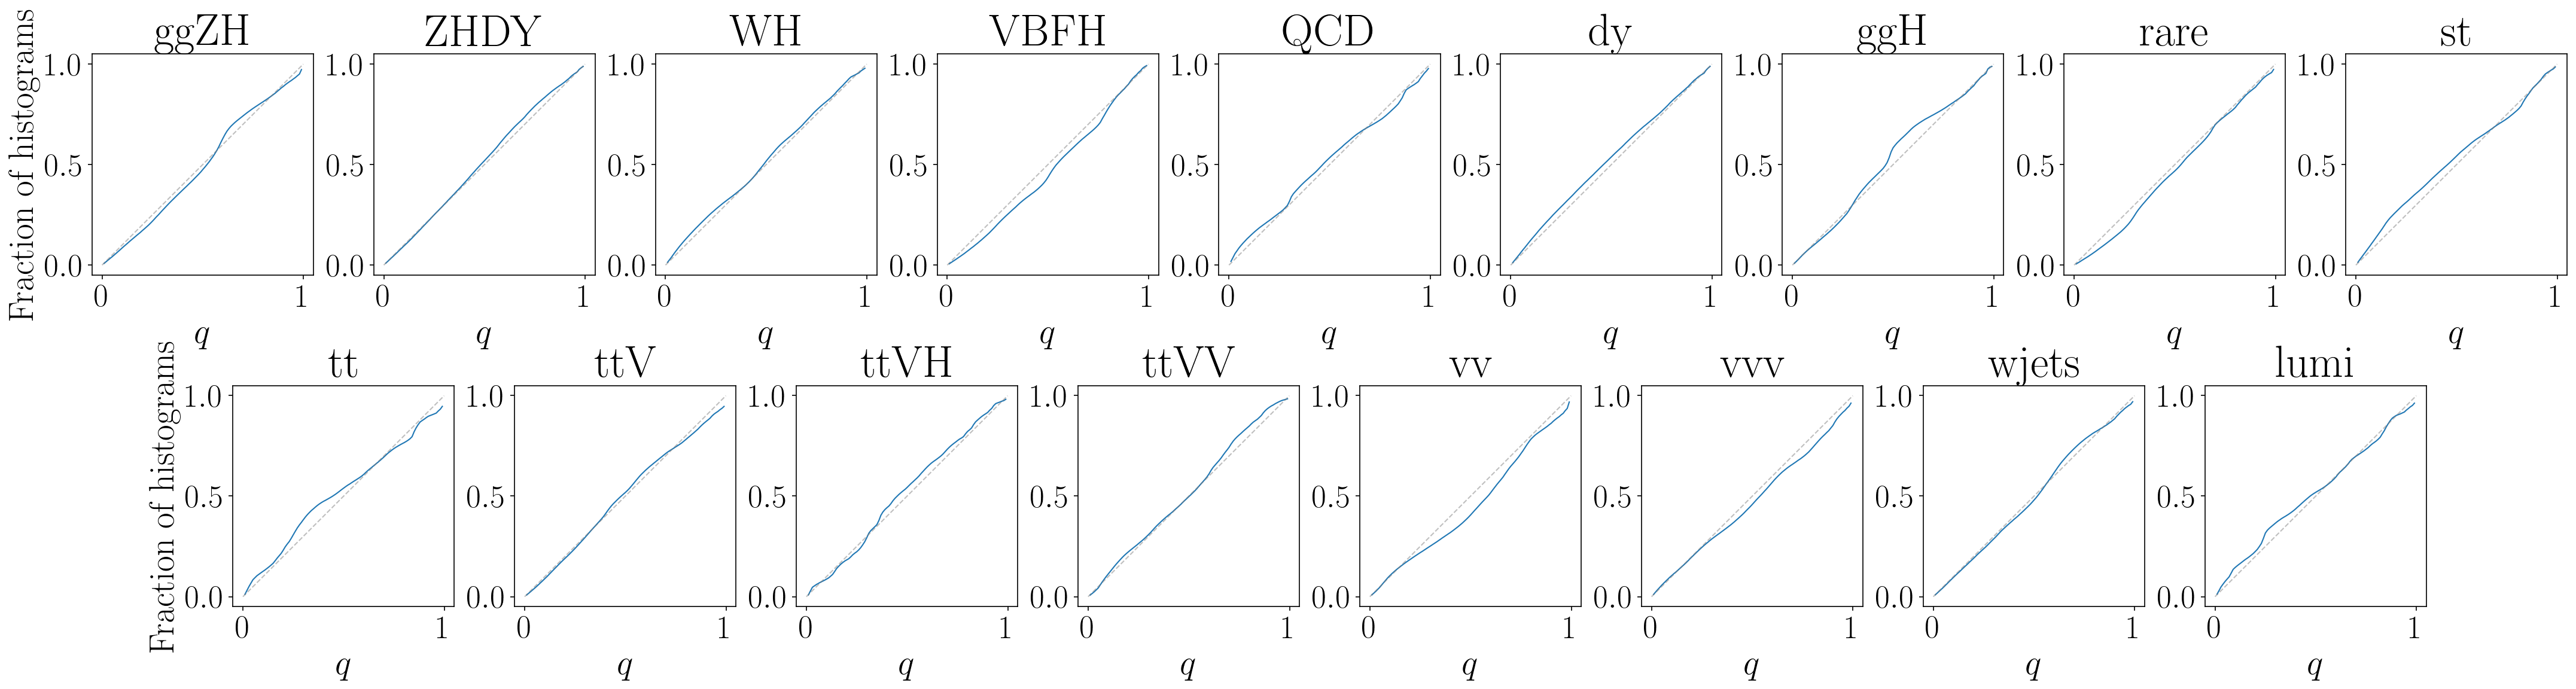
\includegraphics[width=\linewidth]{figures/inference/ecal_SN}
	\caption{\textcolor{red}{Need to be updated!} Note that they are close to the "Urpsrungsgeraden".}
	\label{fig:ecals}
\end{figure}

A natural measure to describe how strongly these biases are present in the network is the meadian calibration error, defined as

\begin{equation*}
	e^{med}_{cal} = \text{med}\left|\frac{N^q_{in}}{N} - q\right|
\end{equation*}

These values for both networks have been listed in tab. \ref{tab:ecal_med}. As it can be seen from the table all of these values are $e^{med}_{cal}\lesssim\mathcal{O}(0.04)$. With such small mean deviations and calibration curves being close to the unit line $x=y$, the resulting network model has no significant inherent biases (due to wrong initialization or other effects).

\begin{table}[h!]
	\centering
	\begin{tabular}{ccc}
		\multirow{2}{*}{Process}& \multicolumn{2}{c}{$e^{med}_{cal}$} \\
		 & cINN & SN-cINN \\
		\hline
		\texttt{ggZH }   & 0.0156    &    0.0258  \\
		\texttt{ZHDY }   & 0.0299    &    0.0103  \\
		\texttt{WH   }   & 0.0148    &    0.0176  \\
		\texttt{VBFH }   & 0.0256    &    0.0428  \\
		\texttt{QCD  }   & 0.0147    &    0.0285  \\
		\texttt{dy   }   & 0.0133    &    0.0323  \\
		\texttt{ggH  }   & 0.0395    &    0.0183  \\
		\texttt{rare }   & 0.0399    &    0.0261  \\
		\texttt{st   }   & 0.0229    &    0.0323  \\
		\texttt{tt   }   & 0.0101    &    0.0300  \\
		\texttt{ttV  }   & 0.0212    &    0.0144  \\
		\texttt{ttVH }   & 0.0159    &    0.0227  \\
		\texttt{ttVV }   & 0.0403    &    0.0146  \\
		\texttt{vv   }   & 0.0333    &    0.0441  \\
		\texttt{vvv  }   & 0.0326    &    0.0331  \\
		\texttt{wjets}   & 0.0070    &    0.0127  \\
		\texttt{lumi }   & 0.0156    &    0.0248  \\
		\hline
	\end{tabular}
	\caption{The median calibration errors for the cINN and the summary network-extended (SN-cINN).}
	\label{tab:ecal_med}
\end{table}

\Subsection{\textcolor{red}{Network Predictions}}

\Subsection{\textcolor{red}{Benchmark Comparison}}